\documentclass[10pt]{article}
\usepackage{icmlko}

\icmlmeta{IP 파운데이션 월드모델}{330}{다시 재니 자가 멀쩡했다}{노트 328의 표를 올바른 마스크로 다시 쟀다 --- 세 주장 중 둘이 오염이었고 하나가 남는다}

\begin{document}

\twocolumn[
\icmlheader

\begin{abstract}
노트 329가 노트 328의 재추출 마스크에 결함이 있다고 적고 다시 재겠다고
했다. 다 쟀다. \textbf{세 주장 중 둘이 무너지고 하나가 남는다.}

\textbf{무너진 것 ①} ``학습 잡음은 표본 수를 안 따른다''. \textbf{따른다.}
정정하면 학습SE 가 $0.55/\sqrt{n}$ 위에 거의 그대로 앉는다 --- 웹툰(711)
0.0171 · 애니(606) 0.0191 · 세계애니(300) 0.0095 · 아이돌(25) 0.1093.
짝SE 대비 비도 2$\sim$8배가 아니라 \textbf{0.86$\sim$4.27} 이고 세계애니는
\textbf{1보다 작다}.

\textbf{무너진 것 ②} ``도메인 순서가 이웃 0/5 로 안 선다''. 정정하면
\textbf{13/15 · 이웃 3/5 · ``순서 선다''} 다. 짝SE 만 쓸 때(14/15 · 이웃
4/5)와 거의 같다.

\textbf{남는 것} \textbf{학습 잡음은 채점 잡음보다 크다} --- 여섯 중 다섯이
1.45$\sim$4.27 배다. 그리고 \textbf{판은 안 흔들린다}: 판 학습SE 가
\textbf{0.0085} 로 미결정 폭 0.010 \emph{아래}다.

\textbf{그리고 새로 하나.} 같은 자료 · 같은 뽑기로 정식화 셋을 돌리니
\textbf{챔피언이 제일 작은 도메인에서 3$\sim$4배 흔들린다} --- 아이돌
학습SE 가 F18 배깅부스트 \textbf{0.1093} 대 F6 직접풀링 0.0366 대 F10
개별수축 \textbf{0.0292}. 판 $\rho$ 는 F18 이 확실히 앞서지만(0.4681 대
0.4323 · 폭 밖), \textbf{흔들림은 F18 이 판에서도 두 배}(0.0085 대 0.0046)다.
\textbf{자료가 아니라 정식화가 바닥을 정한다.}

덤으로 잡음의 출처도 갈랐다 --- 웹툰만 재추출 0.0135 · 남 아홉만 0.0084 ·
제곱합 0.0159 이 전부 재추출한 0.0171 과 맞는다. \textbf{두 원천은 독립이고
가법이다.} 다만 ``작을수록 남에게 흔들린다''는 \textbf{안 나온다} ---
몫이 26\%$\sim$81\% 인데 크기와 아무 관계가 없다(아이돌 37\% · 애니 26\% ·
시장팝업 81\%).
\end{abstract}
]

\section{무엇이 오염이었나}

노트 328의 재추출 함수가 학습 행을 \texttt{dom[d][3] < 2025} 로 골랐다.
일곱 도메인에서 그 배열은 로그 경과시간(0.8$\sim$4.1)이라 \emph{모든} 행이
학습으로 잡혔고 \textbf{유보까지 재추출됐다.} 그래서 ``학습SE''에 채점
잡음이 통째로 섞였다. 이번에는 \texttt{Data.rows(post=True, labeled=True)}
로 자른다(노트 329에 붙인 \texttt{Data.weights} 도 같은 자리).

\begin{figure*}[t]
\centering
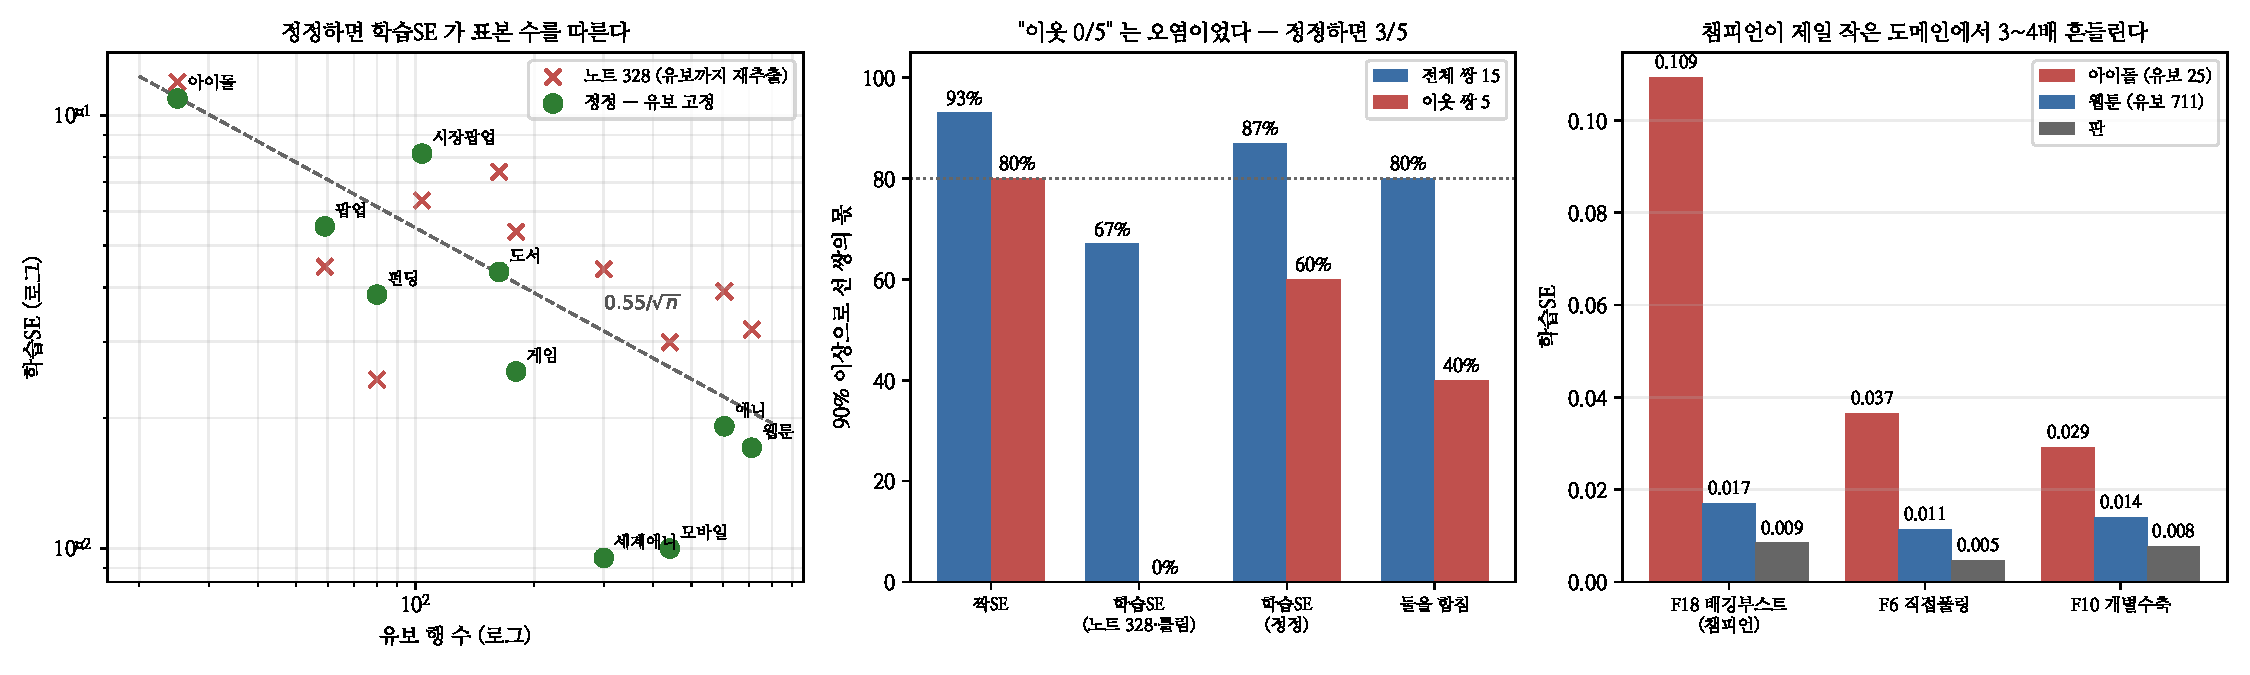
\includegraphics[width=\textwidth]{figs/remeasure.pdf}
\caption{왼쪽 --- 학습SE 와 유보 크기. 가운데 --- 순서가 몇 쌍이나 서나.
오른쪽 --- 정식화별 학습SE.}
\end{figure*}

\section{표를 다시 낸다}

F18 배깅부스트 · \texttt{trendcalwikitag} · $t15$ · 뽑기 스물넷.

\begin{center}\footnotesize
\begin{tabular}{lrrrrr}
\hline
도메인 & 유보 & 학습SE & 짝SE & 비 & 328 \\
\hline
게임 & 180 & 0.0256 & --- & --- & 0.0538 \\
모바일 & 441 & 0.0100 & 0.004 & 2.50 & 0.0299 \\
세계애니 & 300 & 0.0095 & 0.011 & \textbf{0.86} & 0.0441 \\
애니 & 606 & 0.0191 & 0.006 & 3.19 & 0.0392 \\
웹툰 & 711 & 0.0171 & 0.004 & 4.27 & 0.0320 \\
팝업 & 59 & 0.0554 & --- & --- & 0.0447 \\
도서 & 163 & 0.0435 & 0.030 & 1.45 & 0.0740 \\
시장팝업 & 104 & 0.0816 & --- & --- & 0.0635 \\
펀딩 & 80 & 0.0385 & --- & --- & 0.0245 \\
아이돌 & 25 & \textbf{0.1093} & 0.056 & 1.95 & 0.1192 \\
\hline
\textbf{판} & 2,675 & \textbf{0.0085} & --- & --- & 0.0308 \\
\hline
\end{tabular}
\end{center}

\textbf{잘못 잰 값이 대개 두 배쯤 컸다} --- 유보를 같이 흔들었으니
당연하다. 그리고 \textbf{작은 도메인일수록 덜 부풀었다}(아이돌 0.1192
$\to$ 0.1093)는 것도 앞뒤가 맞는다. 아이돌은 \texttt{t} 가 진짜 연도라
그 도메인만 원래 옳게 잘리고 있었다.

\paragraph{판은 안 흔들린다} 판 학습SE 0.0085 가 미결정 폭 0.010
\emph{아래}다. 노트 329가 짝지은 차로 이미 본 것과 같다(축만 0.0016 ·
행까지 0.0055). \textbf{폭 0.010 은 넉넉하다.}

\section{남는 주장 하나}

\begin{center}\small
\begin{tabular}{lr}
\hline
학습SE $>$ 짝SE 인 도메인 & \textbf{5/6} \\
비 범위 & 0.86 $\sim$ 4.27 \\
\hline
\end{tabular}
\end{center}

\textbf{학습 쪽이 더 크다는 것 자체는 맞았다.} 다만 ``2$\sim$8배''가 아니라
``대개 1.5$\sim$4배''이고, \textbf{큰 도메인일수록 비가 크다}는 관찰은
살아 있다(웹툰 4.27 · 애니 3.19 · 모바일 2.50 대 도서 1.45 · 아이돌 1.95).
채점 잡음이 $1/\sqrt{n}$ 으로 더 빨리 줄기 때문이다 --- \textbf{둘 다
표본 수를 따르는데 기울기가 다르다.}

\section{순서는 선다}

\begin{center}\footnotesize
\begin{tabular}{lrr}
\hline
쓴 SE & 선 쌍 & 이웃 \\
\hline
짝SE (노트 316) & 14/15 (93\%) & 4/5 \\
학습SE (노트 328 · 오염) & 10/15 (67\%) & \textbf{0/5} \\
\textbf{학습SE (정정)} & \textbf{13/15 (87\%)} & \textbf{3/5} \\
둘을 합침 & 12/15 (80\%) & 2/5 \\
\hline
\end{tabular}
\end{center}

\textbf{노트 328의 ``이웃이 하나도 안 선다''를 거둔다.} 합쳐도 ``순서
선다'' 문턱(80\%)에 걸린다. 노트 316의 그림은 그대로 두면 된다.

\section{그리고 챔피언이 제일 많이 흔들린다}

같은 자료 · 같은 뽑기(열다섯)로 정식화 셋.

\begin{center}\footnotesize
\begin{tabular}{lrrrr}
\hline
정식화 & 판 & 판SE & 아이돌 & 웹툰 \\
\hline
\textbf{F18 배깅부스트} & \textbf{0.4681} & 0.0085 & \textbf{0.1093} & 0.0171 \\
F6 직접풀링 & 0.4323 & \textbf{0.0046} & 0.0366 & \textbf{0.0114} \\
F10 개별수축 & 0.3955 & 0.0077 & \textbf{0.0292} & 0.0140 \\
\hline
\end{tabular}
\end{center}

\textbf{챔피언 자격은 흔들리지 않는다} --- 판 차 0.036 이 미결정 폭 0.010
밖이다. 그런데 \textbf{그 판을 사는 대가가 흔들림}이다: 아이돌에서 F10 의
\textbf{3.7배}, 판에서 F6 의 \textbf{1.8배}.

\begin{center}\small
\begin{tabular}{ll}
\hline
바닥은 자료의 성질인가 & \textbf{아니다} \\
같은 아이돌 25행에서 & F18 0.1093 · F10 0.0292 \\
\hline
\end{tabular}
\end{center}

\textbf{``이 도메인은 유보가 25행이라 못 잰다''는 반쯤만 맞는 말이었다} ---
정식화를 바꾸면 같은 25행에서 넉 배 덜 흔들린다.

\section{잡음의 출처}

\begin{center}\footnotesize
\begin{tabular}{lrrr}
\hline
흔든 것 & 웹툰 SD & \\
\hline
웹툰만 & 0.0135 & 72\% (분산 몫) \\
남 아홉만 & 0.0084 & 28\% \\
제곱합 & 0.0159 & 전부 0.0171 \\
\hline
\end{tabular}
\end{center}

\textbf{두 원천이 독립이고 가법이다.} 그런데 노트 329를 쓸 때 오염된
수로 본 ``작을수록 남에게 흔들린다''는 \textbf{안 나온다} --- 몫이
아이돌 37\% · 애니 26\% · 시장팝업 81\% · 모바일 52\% 로 크기와 관계가
없다. \textbf{풀링이 잡음을 나눠 갖는 것은 맞지만 크기 규칙은 없다.}

\section{남은 것}
\begin{center}\footnotesize
\begin{tabular}{ll}
\hline
갈래 & 왜 \\
\hline
\textbf{F10 은 왜 아이돌에서 안 흔들리나} & 같은 25행인데 넉 배 \\
흔들림을 이름표로 & 청력 · 겹침과 같은 자리 \\
F18 을 덜 흔들리게 & 배깅을 늘리면 되나 \\
왜 시장팝업이 81\% 인가 & 유일하게 큰 몫 \\
\hline
\end{tabular}
\end{center}

\paragraph{규약} \textbf{오염된 자로 잰 것은 방향까지 뒤집힌다.} 노트 328이
낸 셋 중 둘이 부호까지 반대였다 --- ``표본 수를 안 따른다''(따른다) ·
``이웃이 안 선다''(선다). \textbf{그리고 남은 하나도 크기가 반이 됐다.}
값이 조금 틀린 게 아니라 \emph{다른 것을 재고 있었다.} 그럴 때는 ``대충
맞겠지''가 안 통한다. 그리고 되짚어 보면 신호가 있었다 --- 노트 328의
표에서 \textbf{펀딩(유보 80)이 웹툰(711)보다 SE 가 작았다}(0.0245 대
0.0320). \textbf{말이 안 되는 자리를 말이 되게 읽으려 했던 것}이
``표본 수를 안 따른다''는 주장이었다.

\end{document}
